\documentclass[11pt]{article}
\usepackage[margin=1in]{geometry}
\usepackage{amsmath, amssymb, booktabs, multirow}
\usepackage{graphicx}
\usepackage{hyperref}

\title{Learning Useful GVFs for Streaming RL under Partial Observability and Non-Stationarity}
\author{}
\date{}

\begin{document}
\maketitle

\begin{abstract}
We study when predictive representations learned through general value functions (GVFs) become useful state for replay-free streaming reinforcement learning under partial observability and non-stationarity. Our setting is a continuing delayed-cue control problem where a prediction may be accurate yet still fail to preserve the hidden variable needed for action selection. We build a family of non-stationary T-maze benchmarks with shallow linear agents and tile-coded features, compare hand-designed and automatically generated GVFs, and develop an online GVF bank that encourages complementary predictive roles rather than single-task selection. In a richer big-world benchmark with cue corruption, distractors, and variable junction timing, balanced role-aware GVF generation improves short-horizon adaptation over earlier automatic baselines, and a contextual role-valuation variant becomes the strongest automatic method in the severe-drift regime. At the same time, the moderate regime remains unresolved: trajectory clustering and targeted coupling ablations show that the useful families there require a delicate \texttt{memory-timing + control} composition that our current online coupling rules do not reliably stabilize. Overall, the results separate predictive accuracy from representation usefulness, show that autonomous GVF discovery benefits from explicit structural pressure toward complementarity, and identify joint bank-structure and coupling control as the main remaining bottleneck.
\end{abstract}

\section{Introduction}
Predictive knowledge has long been proposed as a foundation for agent state, but in streaming reinforcement learning the key question is not whether an agent can learn a prediction at all. The harder question is whether the learned prediction becomes \emph{useful state} for control. In partially observable problems a predictive task may be accurate while still discarding the hidden distinction that determines the correct action. Under non-stationarity the gap becomes even sharper: a representation may preserve hidden information yet still fail to support fast adaptation when the decision rule changes.

This paper studies that gap in a deliberately constrained setting. We focus on replay-free continuing control, shallow linear function approximation, and no recurrent network memory. The benchmark is a delayed-cue T-maze in which the agent sees a binary cue at trial start, traverses an aliased corridor, and must act correctly at a later junction. The big-world variants further add cue corruption, distractors, variable junction timing, and changes in the cue-to-action mapping. These conditions let us ask a clean question: when does a GVF-derived representation preserve decision-critical hidden information at action time \emph{and} improve downstream policy learning?

Our empirical story has three parts. First, predictive accuracy and representation usefulness do separate in practice. Stronger cue decodability does not automatically yield better post-switch control, both in early pilot settings and in the richer big-world benchmark. Second, useful automatic GVF discovery requires structure. Moving from single-task selection to a small bank of complementary GVFs, and then to balanced role-aware replenishment, produces the first robust automatic gains in the harder non-stationary settings. In particular, balanced self-improving banks improve short-horizon adaptation in the default big-world benchmark, and contextual role valuation becomes the strongest automatic method in the severe-drift regime. Third, the moderate regime remains unsolved in an informative way. Across structured coupling, family smoothing, and persistent-control variants, the best trajectories consistently require a mixed \texttt{memory-timing + control} composition with intermediate coupling, but our current online rules do not stabilize it.

These results motivate the paper's main claim: useful GVFs in streaming RL are not just accurate predictions, and autonomous GVF discovery is not just a search problem over cumulants and horizons. What matters is whether predictive tasks induce a bank structure that preserves hidden information, provides complementary timing/control/regime support, and couples to control with the right strength under drift. The rest of the paper develops this claim through progressively richer experiments, ending with severity generalization, role ablations, transfer, and a concrete diagnosis of the current bottleneck.

\section{Related Work}
This work is closest in spirit to research on predictive state and GVFs, where the central idea is that agents can build state through learned forecasts rather than hand-designed latent variables. Our contribution is narrower and more control-focused: we ask when such forecasts become \emph{useful representations} for streaming policy learning under partial observability and non-stationarity, rather than treating prediction learning itself as the endpoint.

The paper is also related to auxiliary-task learning in reinforcement learning. Much of that literature studies whether additional predictive objectives help representation learning, often in deep and replay-based settings. Our setting is intentionally different: linear function approximation, no replay buffer, and continuing online adaptation. This makes the failure cases easier to interpret. A predictive auxiliary can be accurate, decodable, and still not help control.

Finally, our automatic GVF generation experiments connect to broader work on adaptive representations, feature discovery, and non-stationary control. The distinctive choice here is to keep the generation mechanism shallow and interpretable. Instead of learning a black-box latent space, the agent selects and mutates semantically meaningful predictive tasks, maintains a small active bank, and can be analyzed through role occupancy, family clustering, and coupling behavior. This allows us to turn negative results into diagnosis: the unresolved moderate regime is not just a performance gap, but evidence that bank structure and control coupling must likely be learned jointly.

\section{Problem Formulation}
We study a continuing partially observable Markov decision process in which each trial begins with a binary cue, followed by an aliased corridor and a delayed junction decision. Let $o_t$ denote the observation, $a_t$ the action, and $r_t$ the reward. Because the corridor observation aliases the hidden cue, the agent must construct an internal predictive state from streaming experience if it is to act correctly at the junction. Learning is strictly online: there is no replay buffer, no offline fitting stage, and no deep recurrent memory. Both control and prediction use shallow linear function approximation, with either raw features or tile-coded features.

Our base predictive primitives are general value functions
\[
v_g(x_t) \approx \mathbb{E}\!\left[\sum_{k \ge 0} \gamma_g^k c_g(o_{t+k+1}, r_{t+k+1}, i_{t+k+1}) \mid x_t\right],
\]
where $x_t$ is the current feature vector, $c_g$ is the cumulant associated with GVF $g$, and $\gamma_g$ is its horizon parameter. The cumulants considered in this work include hand-designed signals such as \texttt{cue}, \texttt{correct\_turn}, \texttt{time\_to\_junction}, \texttt{mapping\_version}, and mixtures of these that couple memory, timing, and regime information. A control agent acts from either raw observation features alone or a joint feature vector augmented by the current GVF predictions.

We evaluate usefulness along two coupled criteria. The first is \emph{state preservation}: the representation should retain the hidden cue or an equivalent control-relevant latent variable until action time. The second is \emph{control utility}: using the representation should improve policy learning, especially after non-stationary changes. Accordingly, our core metrics are trial accuracy, cue decodability at the junction, cue-alignment margin, and prediction TD error; for non-stationary experiments we additionally track pre-switch accuracy, post-switch accuracy, and recovery trials.

The automatic-discovery problem is to choose or generate a small active bank of GVFs online. The central scientific question is not whether a generator can produce many predictive tasks, but which generated bank structures remain control-useful under the big-world hypothesis, where relevant and irrelevant aspects of the environment drift together.

\section{Method}
Our method is an online GVF-bank learner for streaming control under partial observability. The core idea is to learn not a single auxiliary prediction, but a small bank of semantically complementary GVFs whose joint predictions form a more control-useful state. We present the method in two layers: a base banked generator and a smaller set of adaptive extensions for non-stationary settings.

\subsection{Base method}
\subsubsection{Structured GVF design space}
The base design space contains hand-designed cumulants for distinct semantic roles: hidden-state memory (\texttt{cue}), direct control support (\texttt{correct\_turn}), temporal support (\texttt{time\_to\_junction}, \texttt{junction}), and regime tracking (\texttt{mapping\_version}). To move beyond a fixed dictionary, we also allow sparse mixtures such as cue-plus-timing and cue-plus-control combinations, so that the agent can represent hybrid predictive roles while remaining in an interpretable linear setting.

\subsubsection{Control-oriented GVF scoring}
Each candidate GVF is evaluated online using short-horizon statistics that estimate whether it helps control rather than merely prediction. The scoring rule emphasizes decision gain, decodability gain, uncertainty reduction, TD learnability, novelty, and redundancy:
\begin{equation}
\mathrm{score}(g) =
1.4 \cdot \mathrm{decisionGain}
+ 1.0 \cdot \mathrm{decodabilityGain}
+ 0.8 \cdot \mathrm{uncertaintyReduction}
- 0.7 \cdot \mathrm{tdError}
- 0.4 \cdot \mathrm{redundancy}.
\end{equation}
This is a method choice, not only a diagnostic. It encodes our claim that useful GVFs should be judged by control-relevant retention and adaptation, not by predictive accuracy alone.

\subsubsection{Banked selection and generation}
Rather than selecting a single auxiliary task, the agent maintains a small active bank of GVFs. Selection is diversity-aware: candidates are favored when they cover missing semantic roles relative to the current bank and penalized when they are redundant. Generation proceeds through lightweight mutation of horizon and step size together with sparse semantic mixing, producing candidates such as cue-plus-timing or control-plus-regime bridges. This gives a constrained form of novelty: the generator explores a structured neighborhood around interpretable predictive abstractions instead of an unrestricted auxiliary-task space.

\subsection{Adaptive variants}
To adapt under drift, we extend the base method in three directions. First, the agent can retune its scoring weights online from recent control quality, recovery, uncertainty, and decodability. Second, it can replenish the candidate pool in a role-aware way, increasing capacity for semantic families that appear useful. Third, it can modulate how strongly GVF predictions are exposed to control. These are not unrelated heuristics; they are increasingly adaptive versions of the same underlying idea, namely that useful predictive state under drift requires both the right bank composition and the right coupling to policy learning. The main text keeps only the strongest adaptive path, while earlier exploratory variants and additional mechanism traces are deferred to the appendix.

\section{Big-World Non-Stationarity}
To move closer to the big world hypothesis, we introduced a richer non-stationary benchmark with three simultaneous perturbation channels:
\begin{itemize}
    \item cue corruption that changes across regimes
    \item stochastic distractor observations in the corridor
    \item variable junction timing through changing corridor length
\end{itemize}

This setting is intentionally harsher than the earlier mapping-flip benchmark: the agent must preserve useful memory, ignore irrelevant variation, and stay responsive to regime-dependent changes in when and how the cue matters.

This section contains the main empirical contribution of the paper. The central retained results are:
the base banked method outperforms earlier automatic methods and strong simple baselines in the richer benchmark; bank-size and heuristic ablations identify diversity-aware complementarity as the key ingredient; adaptive variants improve automatic adaptation further in some regimes, especially severe drift; and the unresolved moderate regime is best explained as a failure of current coupling-aware extensions rather than a failure of candidate generation alone.

\subsection{Validating the base banked method}
Table~\ref{tab:bigworld} summarizes a four-seed comparison.

\begin{table}[h]
\centering
\begin{tabular}{lcccc}
\toprule
Method & Mean Accuracy & Mean Decodability & Mean Post-switch Acc. & Mean Recovery \\
\midrule
Adaptive bank & 0.5070 & 0.7294 & 0.5565 & 11.25 \\
Adaptive evolution & 0.4955 & 0.6483 & 0.4950 & 12.85 \\
Adaptive selection & 0.5136 & 0.5979 & 0.5043 & 14.25 \\
Raw observation & 0.5065 & 0.5644 & 0.5073 & 14.68 \\
Cue GVF & 0.5087 & 0.5789 & 0.5246 & 12.87 \\
Cue + junction GVF & 0.4917 & 0.5888 & 0.4955 & 11.97 \\
\bottomrule
\end{tabular}
\caption{Big-world non-stationary summary from \texttt{results/bigworld\_method\_summary.csv}.}
\label{tab:bigworld}
\end{table}

The main pattern changed after introducing a diversity-constrained bank. The automatic method now achieves the best overall big-world adaptation result in this comparison: mean post-switch accuracy rises to 0.5565 and mean recovery drops to 11.25, while mean cue decodability increases to 0.7294. This is the first setting in our current study where automatically generated GVFs do not merely improve representation quality, but also outperform the strongest hand-designed and raw baselines on downstream control.

\begin{figure}[h]
\centering
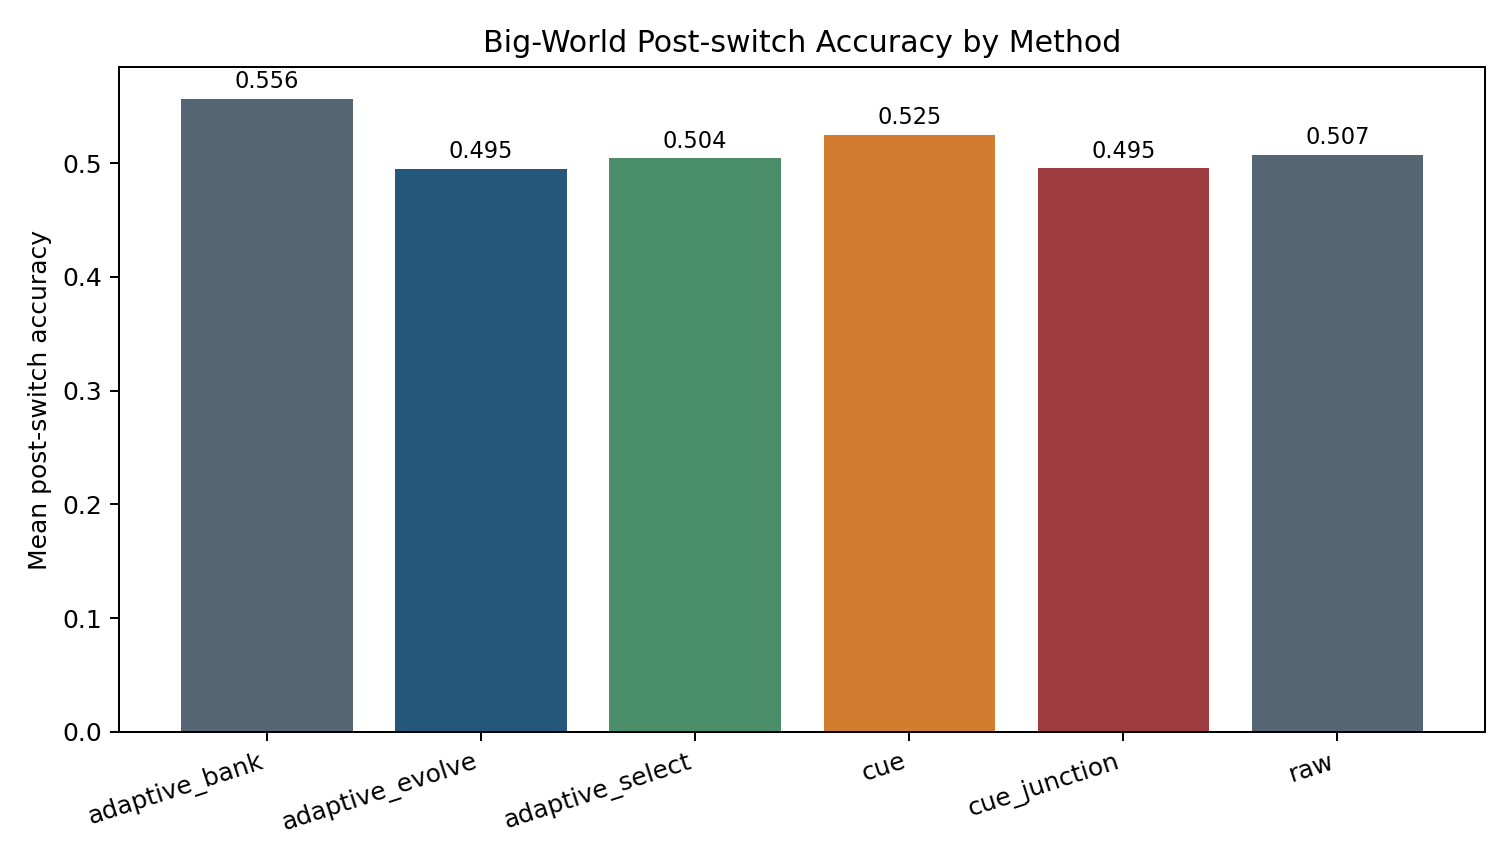
\includegraphics[width=0.8\linewidth]{figures/bigworld_method_postswitch.png}
\caption{Mean post-switch accuracy under richer big-world drift.}
\label{fig:bigworld_method_postswitch}
\end{figure}

\subsection{Ablating base-method components}
We also ran a focused ablation to test two questions:
\begin{enumerate}
    \item How large should the active GVF bank be?
    \item Which heuristic terms are actually responsible for the gain?
\end{enumerate}

Table~\ref{tab:bankablation} summarizes the main result.

\begin{table}[h]
\centering
\begin{tabular}{lcccc}
\toprule
Method & Mean Accuracy & Mean Decodability & Mean Post-switch Acc. & Mean Recovery \\
\midrule
Bank $k=2$ full & 0.4955 & 0.6483 & 0.4950 & 12.85 \\
Bank $k=3$ full & 0.5070 & 0.7294 & 0.5565 & 11.25 \\
Bank $k=4$ full & 0.5148 & 0.7386 & 0.5408 & 13.88 \\
Bank $k=3$, no diversity & 0.4997 & 0.6951 & 0.5196 & 14.00 \\
Bank $k=3$, no novelty & 0.5070 & 0.7294 & 0.5565 & 11.25 \\
Bank $k=3$, no similarity penalty & 0.4948 & 0.7296 & 0.5371 & 11.00 \\
\bottomrule
\end{tabular}
\caption{Bank-size and heuristic ablations from \texttt{results/bank\_ablation\_summary.csv}.}
\label{tab:bankablation}
\end{table}

Three conclusions stand out.
A bank of size $3$ is clearly better than size $2$, which supports the hypothesis that a single auxiliary GVF is not enough under rich non-stationarity. Increasing to size $4$ further improves decodability but hurts post-switch control relative to size $3$, suggesting harmful redundancy or interference in over-complete banks. Most importantly, removing the diversity bonus causes a large drop in both post-switch accuracy and recovery, while removing the novelty bonus has essentially no effect in the current implementation. The main driver of the breakthrough is therefore not novelty by itself, but \emph{diversity-aware complementarity}.

\begin{figure}[h]
\centering
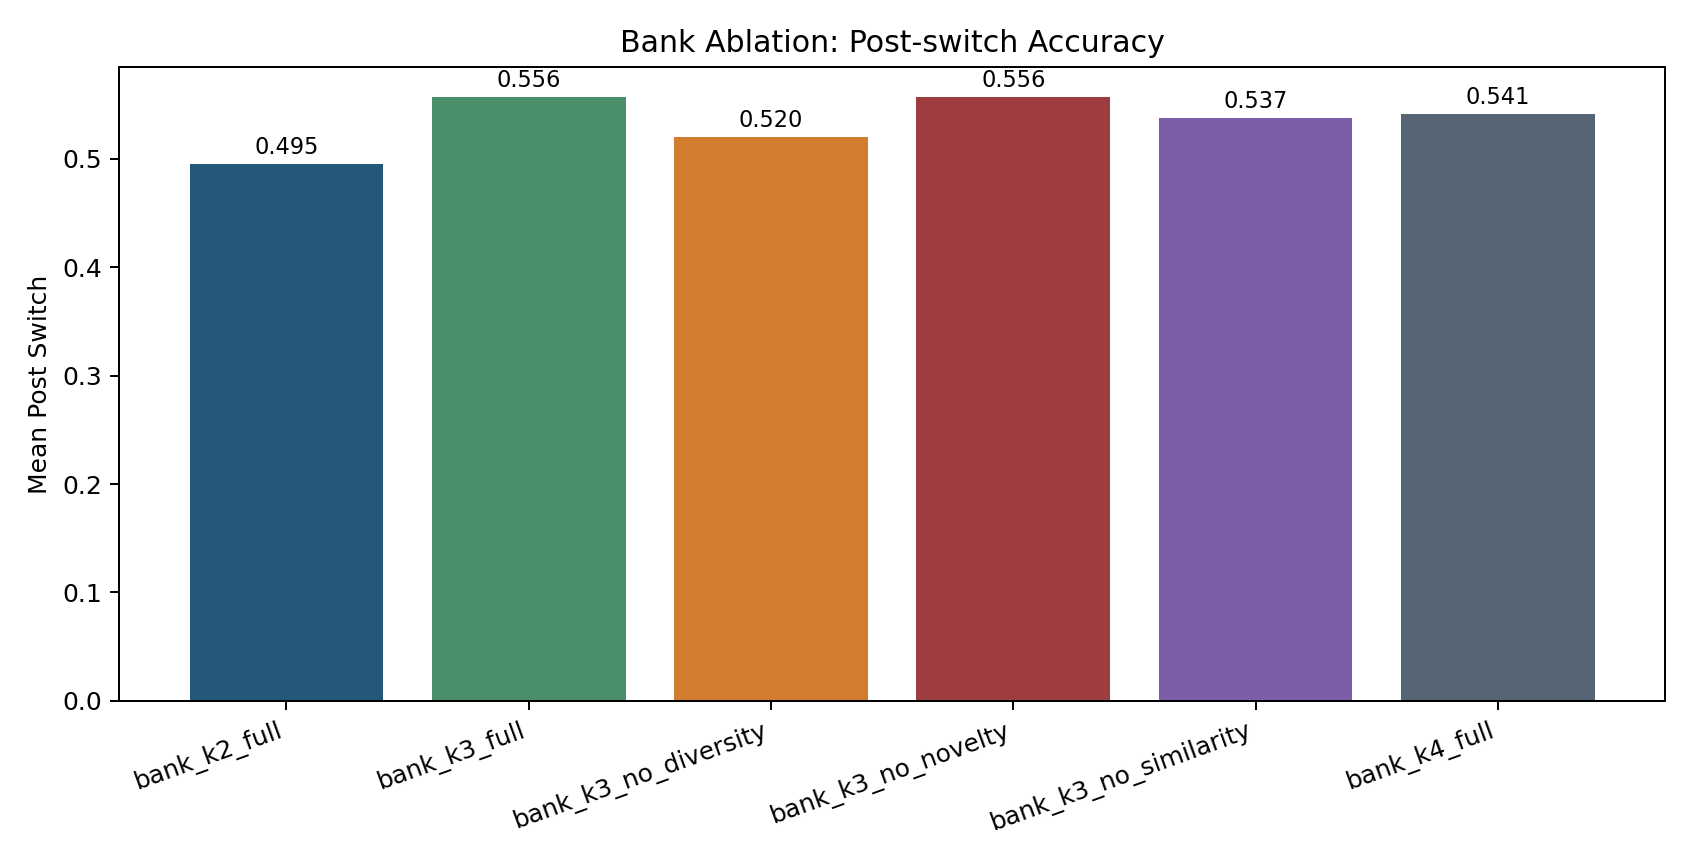
\includegraphics[width=0.8\linewidth]{figures/bank_ablation_postswitch.png}
\caption{Post-switch adaptation for bank-size and heuristic ablations.}
\label{fig:bank_ablation_postswitch}
\end{figure}

\begin{figure}[h]
\centering
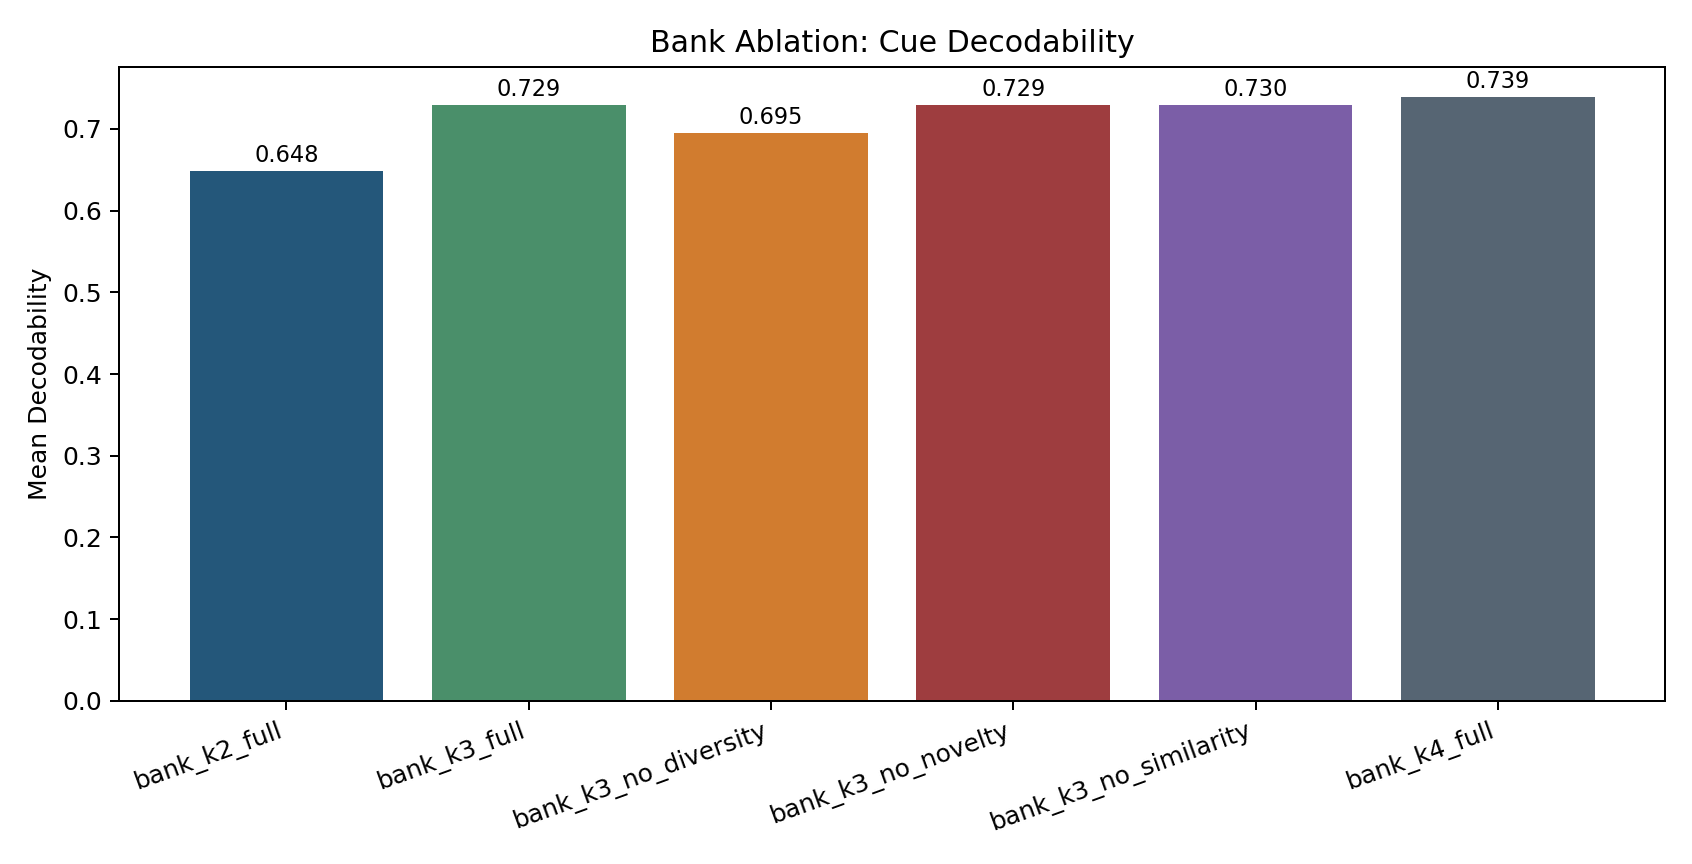
\includegraphics[width=0.8\linewidth]{figures/bank_ablation_decodability.png}
\caption{Cue decodability for bank-size and heuristic ablations.}
\label{fig:bank_ablation_decodability}
\end{figure}

\subsection{Validating adaptive scoring}
The previous ablations compared fixed heuristic components. We next ask a different question: can the agent improve adaptation by changing \emph{how} it scores candidate GVFs while learning proceeds? Table~\ref{tab:metaheuristic} summarizes a four-seed comparison among three fixed heuristic profiles and the new online-retuned meta-heuristic profile.

\begin{table}[h]
\centering
\begin{tabular}{lcccc}
\toprule
Method & Mean Accuracy & Mean Decodability & Mean Post-switch Acc. & Mean Recovery \\
\midrule
Info-gain profile & 0.4873 & 0.7089 & 0.4179 & 14.12 \\
Uncertainty profile & 0.4940 & 0.7039 & 0.4833 & 14.79 \\
Adaptation profile & 0.4866 & 0.7292 & 0.4508 & 12.00 \\
Online meta-heuristic & 0.5309 & 0.7032 & 0.5154 & 12.50 \\
\bottomrule
\end{tabular}
\caption{Fixed-heuristic versus online-retuned heuristic comparison from \texttt{results/meta\_heuristic\_summary.csv}.}
\label{tab:metaheuristic}
\end{table}

The key result is that the online-retuned profile achieves the best mean trial accuracy and the best mean post-switch adaptation, even though it does not maximize cue decodability. The fixed adaptation-biased profile reaches the highest decodability, but its control performance is clearly worse than the meta-heuristic. This gives a second direct demonstration, beyond the role ablations, that better hidden-state decoding is not enough. The agent must also learn when to stop rewarding prediction quality alone and shift pressure toward decision usefulness.

The learned weight traces make this interpretation concrete. In easy windows the meta-heuristic stays close to its initialization. In harder windows it increases decision-gain and adaptation-gain weights while slightly reducing pure decodability emphasis. This changes the active bank in some seeds, preserving timing-support mixtures where the fixed adaptation profile collapses toward a nearly homogeneous bank. The method lesson is that autonomous GVF generation may require two adaptive layers: adapting the bank itself, and adapting the scoring rule used to judge that bank.

\begin{figure}[h]
\centering
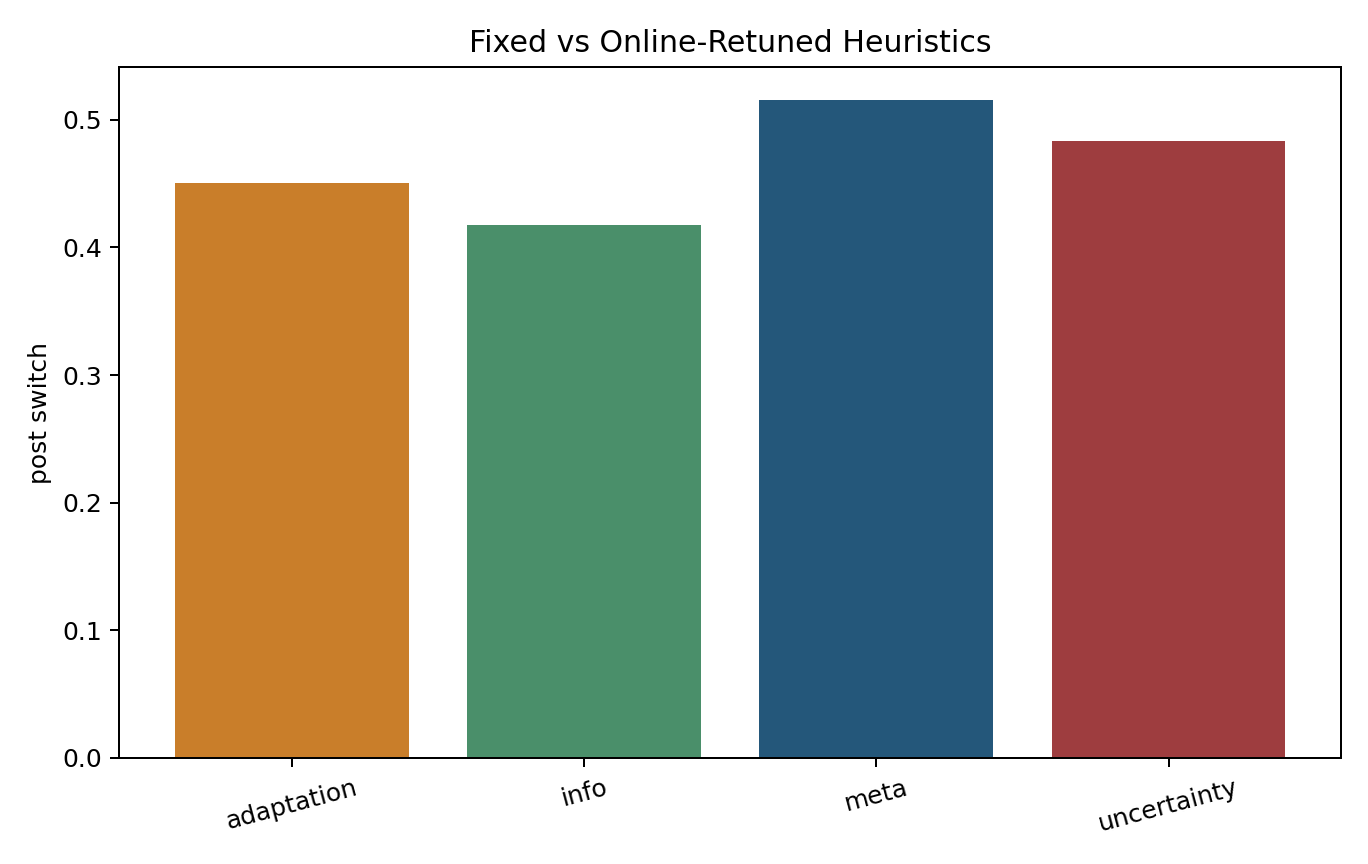
\includegraphics[width=0.8\linewidth]{figures/meta_heuristic_postswitch.png}
\caption{Post-switch accuracy under fixed heuristic profiles versus online heuristic retuning.}
\label{fig:meta_heuristic_postswitch}
\end{figure}

\begin{figure}[h]
\centering
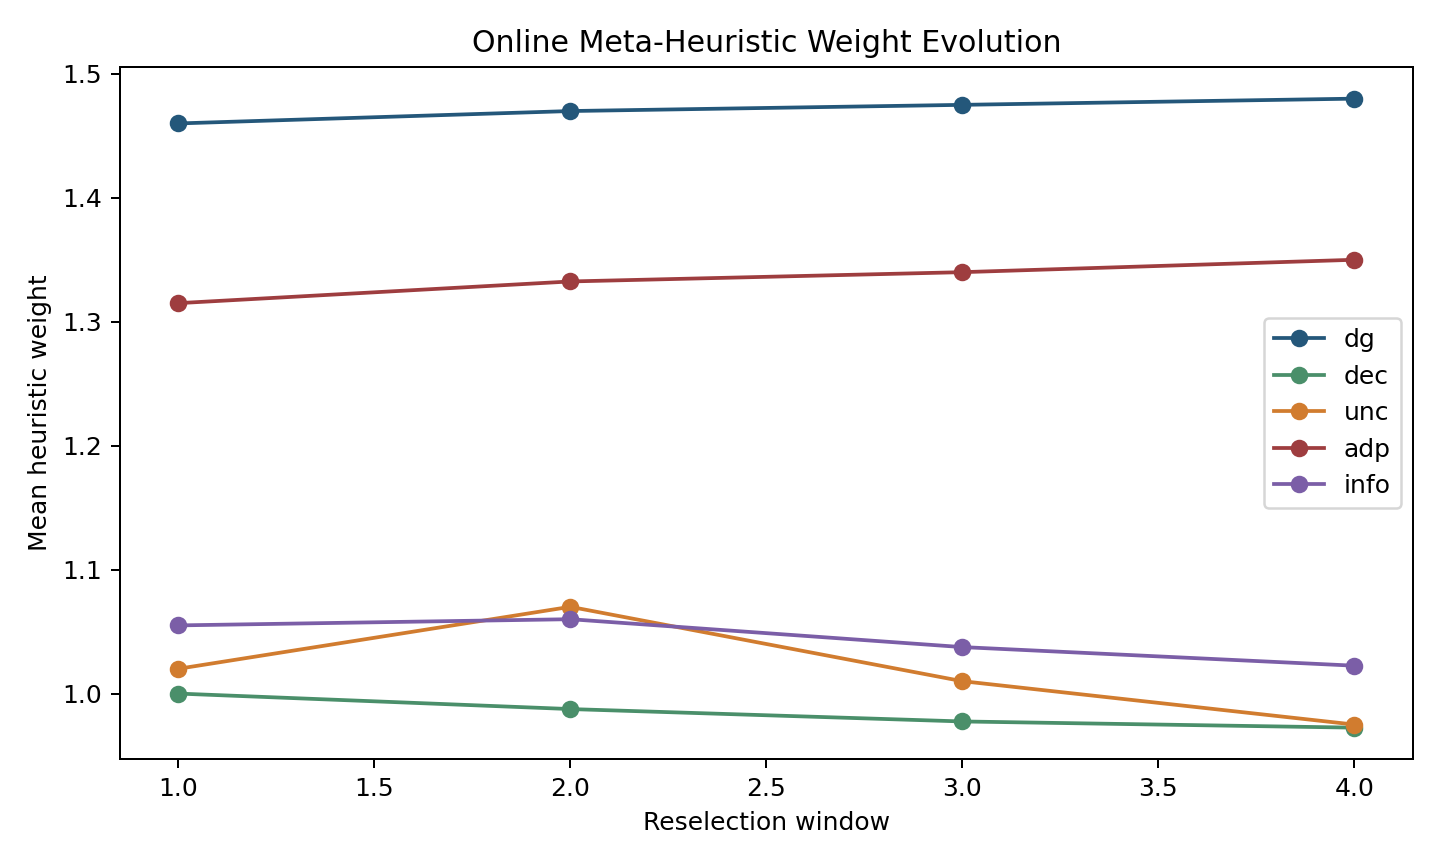
\includegraphics[width=0.78\linewidth]{figures/meta_heuristic_weights.png}
\caption{Mean weight evolution of the online meta-heuristic across reselection windows.}
\label{fig:meta_heuristic_weights}
\end{figure}

\subsection{Testing whether the base method generalizes across severity}
To test whether the learned bank structure reflects a real adaptation principle rather than overfitting a single setting, we evaluated the strongest banked method across a three-level big-world severity sweep. The severity levels vary corridor length, distractor rate, and cue corruption intensity.

\begin{table}[h]
\centering
\begin{tabular}{lccc}
\toprule
Severity & Method & Mean Post-switch Acc. & Mean Decodability \\
\midrule
Mild & Raw / Cue / Bank & 0.4985 / 0.5157 / 0.5135 & 0.5655 / 0.5792 / 0.6689 \\
Moderate & Raw / Cue / Bank & 0.5073 / 0.5246 / 0.5565 & 0.5644 / 0.5789 / 0.7294 \\
Severe & Raw / Cue / Bank & 0.5333 / 0.5009 / 0.5354 & 0.5650 / 0.5997 / 0.7396 \\
\bottomrule
\end{tabular}
\caption{Generalization of the learned GVF bank across drift severity, from \texttt{results/bigworld\_sweep\_summary.csv}.}
\label{tab:severitysweep}
\end{table}

The trend is nuanced but encouraging. In the mild regime the hand-designed cue baseline is still strongest on control, even though the bank has much better representation quality. In the moderate regime the bank clearly dominates both raw observation and the cue baseline. In the severe regime the bank remains competitive with the raw baseline while preserving a much stronger hidden-state representation than either comparator. The main point is not that one method uniformly wins everywhere, but that the learned bank remains useful across a range of drift intensities and shows its clearest advantage when the environment is hard but still structured enough for predictive state to matter.

\begin{figure}[h]
\centering
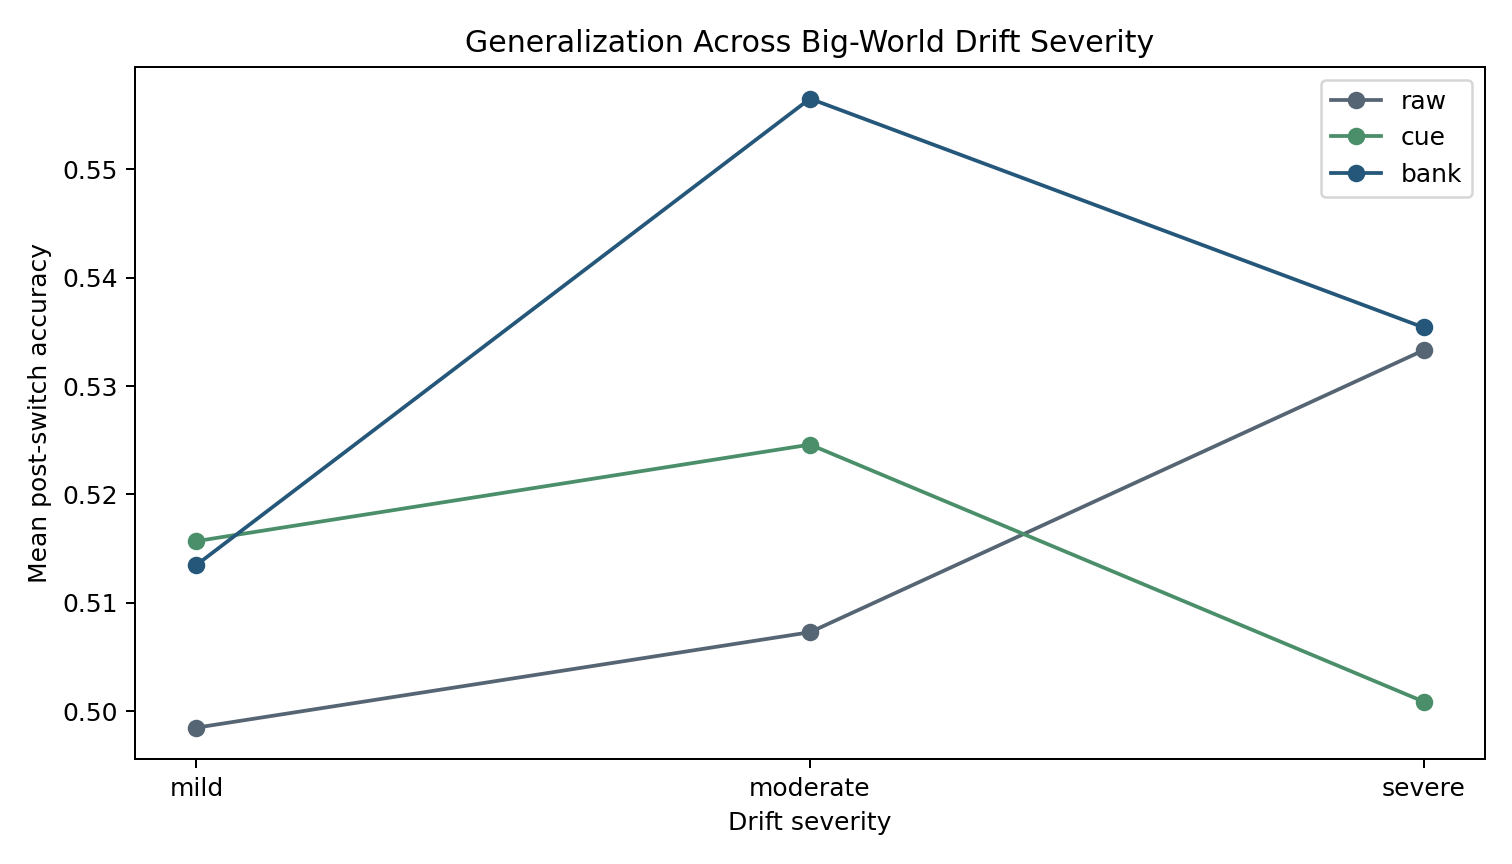
\includegraphics[width=0.8\linewidth]{figures/bigworld_severity_generalization.png}
\caption{Generalization of raw, hand-designed, and banked GVF methods across big-world drift severity.}
\label{fig:severity_generalization}
\end{figure}

\subsection{Testing role-aware and contextual adaptive variants}
We next test a stronger adaptive hypothesis: beyond selecting diverse GVFs, the agent may also need to learn \emph{which semantic roles matter in which worlds}. A first role-value version produced an informative failure. It learned a strong preference for memory-timing mixtures, but often collapsed too aggressively onto that family and dropped to 0.4625 mean post-switch accuracy in a three-seed big-world comparison. This shows that simply learning ``which role matters'' is not enough; without explicit pressure toward complementarity, the agent can over-commit to one useful-looking family too early.

We therefore added a \emph{balanced self-improving bank} that keeps the same online role-value mechanism but regularizes replenishment toward at least one contrastive role family beyond the top-ranked pair. This anti-collapse rule changes the picture substantially. In the same three-seed comparison, the balanced self-improving bank reaches 0.5617 mean post-switch accuracy with 10.27 recovery trials, outperforming all automatic baselines in short-horizon adaptation while remaining fully online and replay-free. We then replaced the hand-shaped role-value update with a tiny contextual bandit. In a two-seed severity sweep, the resulting contextual self-improving bank becomes the best automatic method in the severe regime, reaching 0.6212 mean post-switch accuracy with 0.8661 cue decodability, but it still fails in the moderate regime. The combined lesson is that role-aware generation helps when it is coupled to an explicit prior for complementarity, yet even contextual role valuation does not by itself solve the finer balance required in the moderate world.

\subsection{Diagnosing the coupling failure in the moderate regime}
We then tested several more aggressive moderate-specific coupling ideas, including explicit control-slot preservation, learnable continuous coupling, and discrete coupling rules. All underperformed: in three-seed focused comparisons, the moderate-specific self-improving bank reached only 0.4559 mean post-switch accuracy, the learned-continuous coupling variant fell to 0.3722, and the discrete coupling variant to 0.3762. A final structure-conditioned coupling rule improved the result to 0.5083, bringing it closer to the simpler world-aware meta-bank at 0.5311 but still well below the cue baseline at 0.6111.

The moderate-world trajectory clustering makes the diagnosis precise. The best automatic family is a mixed \texttt{memory-timing + control} pattern with 0.5286 mean post-switch accuracy, 0.6822 decodability, and an intermediate mean coupling strength of 0.67. Timing-only families fall to 0.4733 post-switch accuracy, and timing-plus-uncertainty families to 0.3847. The unresolved moderate regime therefore appears to be a joint bank-structure and coupling problem: useful GVFs there must preserve timing-grounded memory while adding control contrast at an intermediate coupling level.

\subsection{Role ablations: which roles are causally necessary?}
The occupancy analysis shows which roles are present, but not whether they are necessary. To test causal importance, we reran the strongest banked agent while forbidding one role family at a time: \texttt{memory\_timing}, \texttt{memory\_control}, or \texttt{memory\_core}.

\begin{table}[h]
\centering
\begin{tabular}{lcccc}
\toprule
Severity & Ablation & Mean Post-switch Acc. & Mean Decodability & Mean Recovery \\
\midrule
Moderate & Full bank & 0.5565 & 0.7294 & 11.25 \\
Moderate & No memory\_timing & 0.5000 & 0.6752 & 15.09 \\
Moderate & No memory\_control & 0.4906 & 0.6361 & 15.12 \\
Moderate & No memory\_core & 0.4875 & 0.7198 & 12.88 \\
\midrule
Severe & Full bank & 0.5354 & 0.7396 & 12.08 \\
Severe & No memory\_timing & 0.4785 & 0.7101 & 16.92 \\
Severe & No memory\_control & 0.5292 & 0.6770 & 12.92 \\
Severe & No memory\_core & 0.5312 & 0.7884 & 10.25 \\
\bottomrule
\end{tabular}
\caption{Role-level ablations from \texttt{results/role\_ablation\_summary.csv}.}
\label{tab:roleablation}
\end{table}

These ablations reveal two non-obvious points.
Removing \texttt{memory\_timing} causes the largest control collapse in both moderate and severe regimes, showing that timing support remains causally important even under strong drift. At the same time, removing \texttt{memory\_core} in the severe regime actually raises decodability to 0.7884 without improving post-switch control. This is direct evidence that representation quality and control usefulness can diverge.

\begin{figure}[h]
\centering
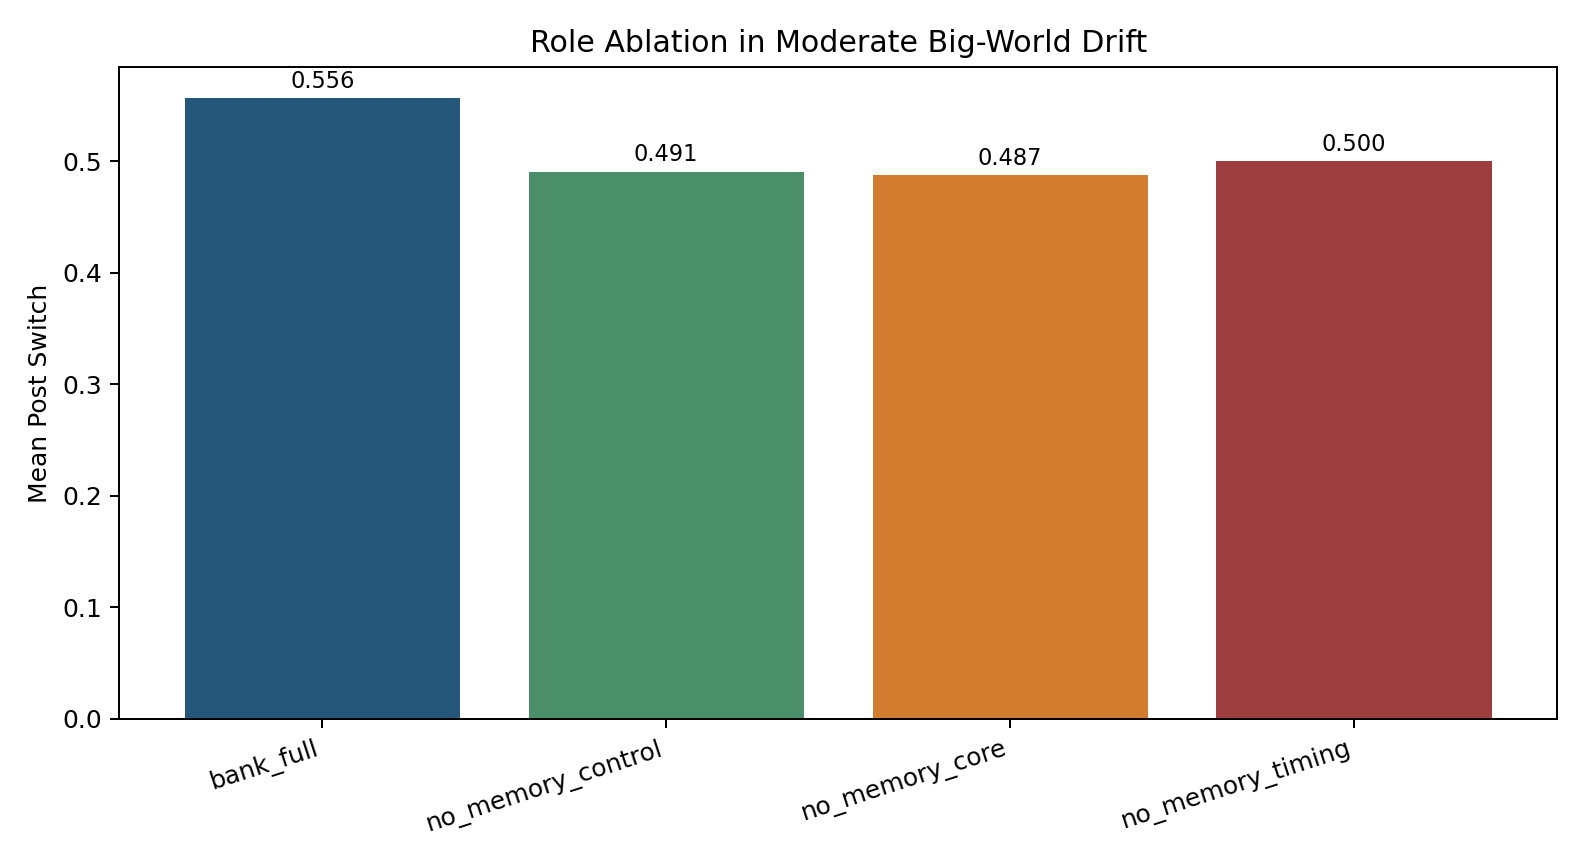
\includegraphics[width=0.8\linewidth]{figures/role_ablation_moderate.png}
\caption{Role ablation results in the moderate big-world regime.}
\label{fig:role_ablation_moderate}
\end{figure}

\begin{figure}[h]
\centering
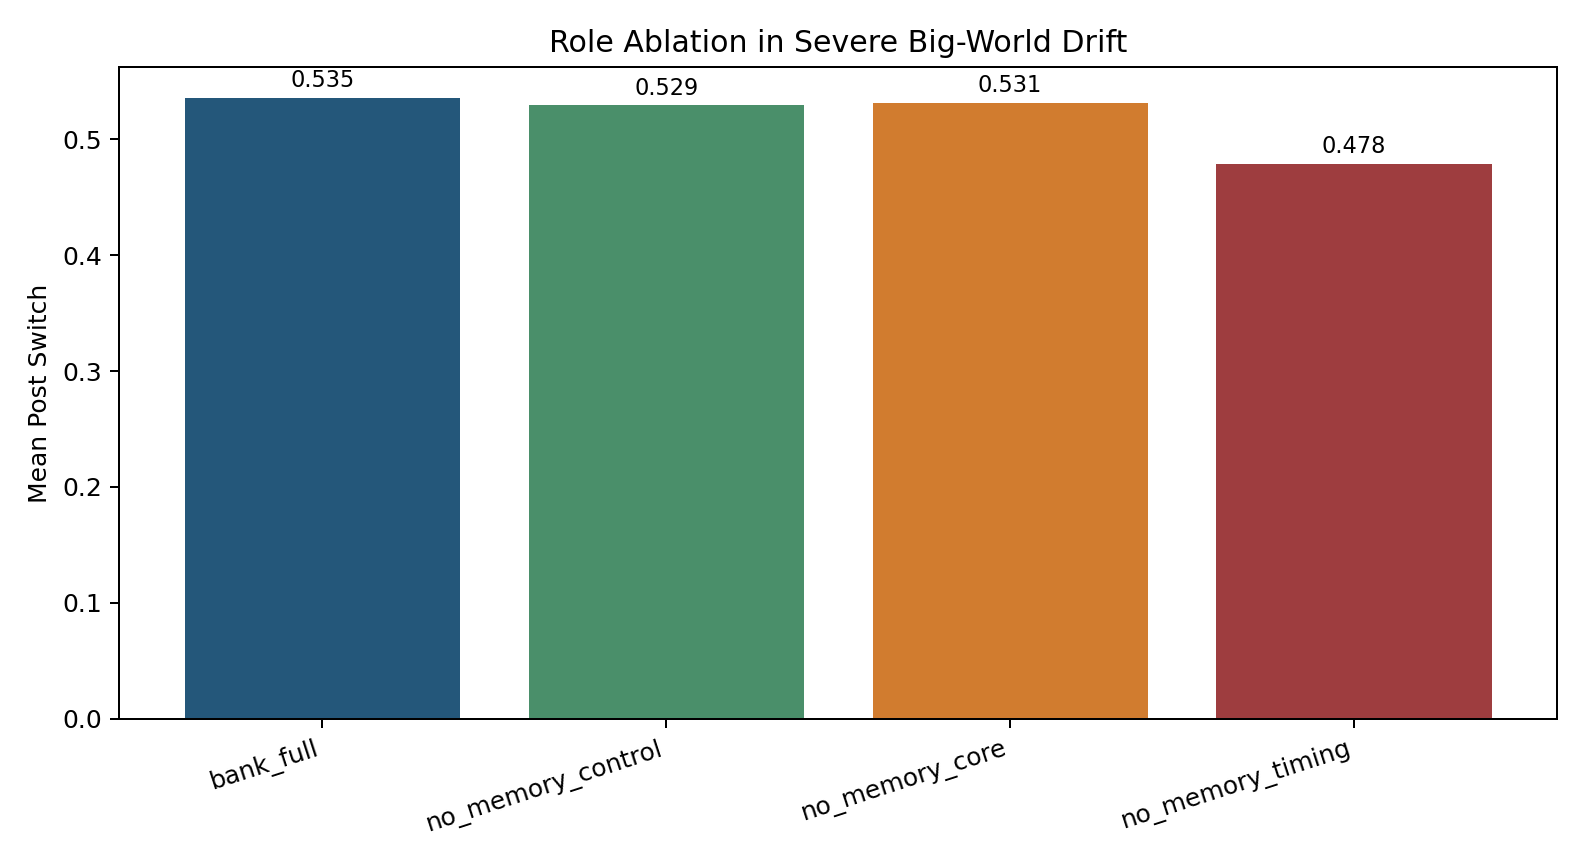
\includegraphics[width=0.8\linewidth]{figures/role_ablation_severe.png}
\caption{Role ablation results in the severe big-world regime.}
\label{fig:role_ablation_severe}
\end{figure}

Taken together, the role occupancy and ablation results suggest a more refined interpretation than ``timing matters less when drift is severe.'' Instead, the bank changes how much of each role it allocates, but timing support remains causally important. What changes is not whether the role matters, but how much bank capacity it deserves relative to core memory and direct control support.

\subsection{Cross-severity transfer}
Finally, we tested whether the learned bank carries predictive structure that remains useful when the environment shifts from a moderate big-world regime to a more severe one without resetting learned weights. This is a stricter test than ordinary within-environment adaptation because the agent must reuse predictive structure acquired under one drift profile while continuing to learn online in a harder regime.

\begin{table}[h]
\centering
\begin{tabular}{lccc}
\toprule
Method & Mean Pre-transfer Acc. & Mean Post-transfer Acc. & Mean Transfer Gap \\
\midrule
Raw observation & 0.4940 & 0.4888 & 0.0053 \\
Cue GVF & 0.5101 & 0.5247 & -0.0146 \\
Adaptive bank & 0.4983 & 0.5769 & -0.0787 \\
\bottomrule
\end{tabular}
\caption{Moderate-to-severe transfer from \texttt{results/transfer\_bigworld\_summary.csv}. Negative transfer gap means the method improves after the transition.}
\label{tab:transfer}
\end{table}

\begin{figure}[h]
\centering
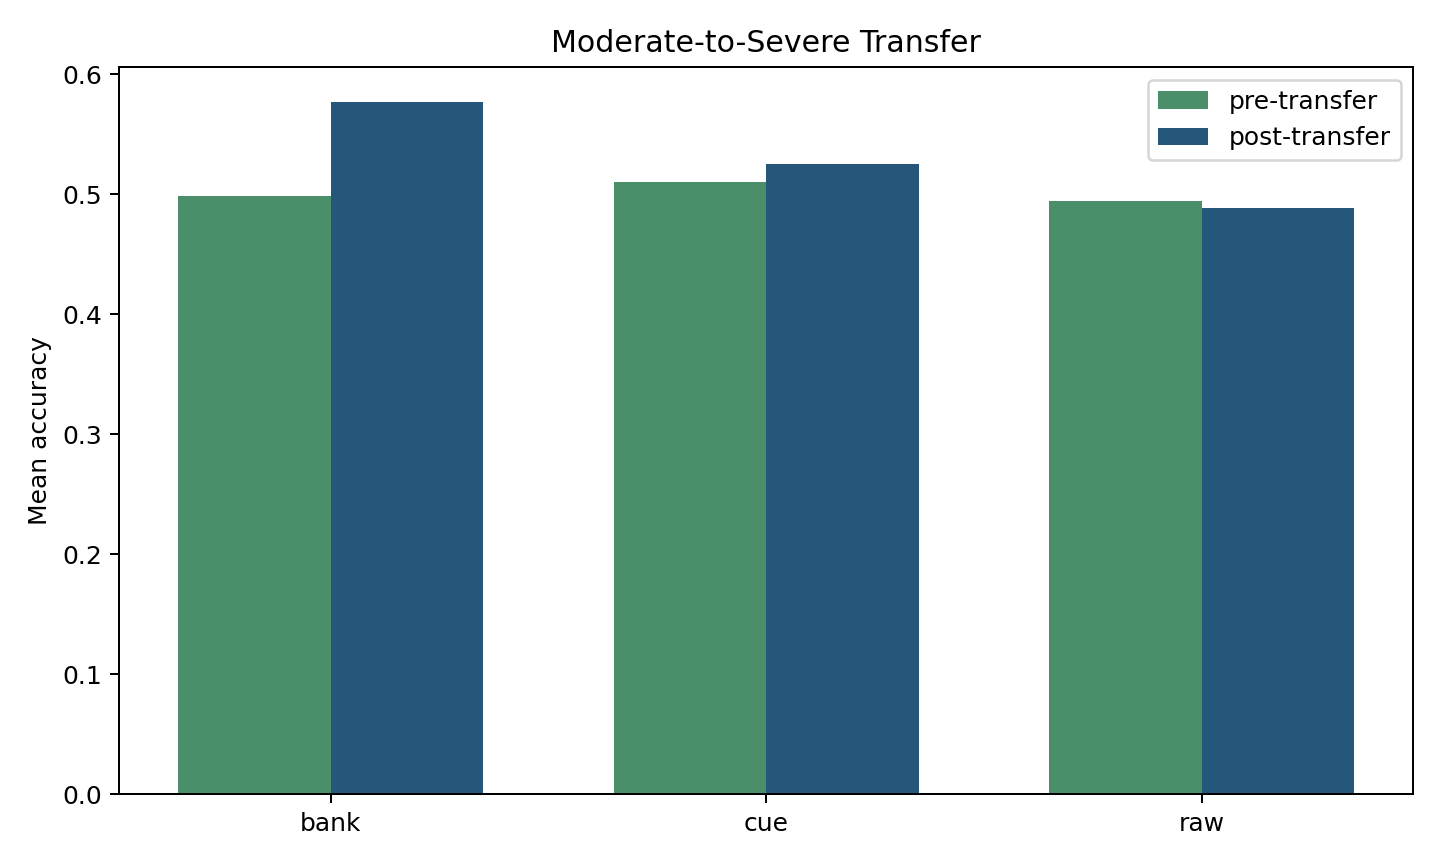
\includegraphics[width=0.76\linewidth]{figures/transfer_bigworld.png}
\caption{Cross-severity transfer from moderate to severe big-world drift.}
\label{fig:transfer_bigworld}
\end{figure}

The banked method improves the most after transfer, reaching 0.5769 mean post-transfer accuracy. This is stronger than the cue baseline and much stronger than raw observation. We interpret this as evidence that the learned GVF bank is not merely overfitting to one particular drift profile. Instead, it appears to carry predictive structure that is reusable when the environment becomes harsher, provided the agent can continue adapting online.

\section{Conclusion}
Our current thesis is:
\begin{quote}
In streaming RL under partial observability and non-stationarity, a useful GVF is one that preserves the hidden distinctions that change the optimal action, tracks the aspects of drift that invalidate old decisions, and can be learned stably online.
\end{quote}

This is a stronger claim than predictive knowledge alone. It says that predictive tasks should be designed or generated to induce a control-ready representation. Our current evidence suggests that such a representation may need a small \emph{bank} structure rather than a single predictive auxiliary: a stable memory-preserving core plus multiple complementary adaptive GVFs for timing and control support. Earlier in the project, novelty was easier to obtain than policy gain; the banked generator is the first evidence in this codebase that structured novelty can be converted into better streaming control under severe non-stationarity. The ablations sharpen this further: the crucial ingredient appears to be diversity-aware functional complementarity, not novelty alone. The severity sweep and role ablations then show that the bank is not static: useful predictive roles reorganize systematically as the environment becomes more unstable, yet timing support remains causally important even when its occupancy share declines.

\section{Discussion}
Four broader lessons emerge from the current study. First, prediction is not enough: a GVF can be learnable and decodable yet still fail to improve control unless it participates in the right predictive division of labor. Second, autonomous generation needs structural pressure: in our experiments, novelty by itself is weak, whereas diversity-aware complementarity is what turns generated predictions into useful control state. Third, useful predictive state is adaptive in composition, not just in value. As the environment becomes harsher, the learned bank changes how much capacity it gives to memory, timing, and control support. Finally, the transfer result suggests that a good predictive bank can carry reusable structure into a harder regime, where continued online learning then amplifies the benefit.

\section{Limitations and Future Directions}
The current study still has several limitations.
\begin{itemize}
    \item The environments are intentionally simple and controlled. They are useful for mechanism discovery, but they are still far from the full complexity implied by the big world hypothesis.
    \item The current generator relies on hand-designed semantic structure in its mutation space and scoring features. A more ambitious version would learn richer candidate-generation operators online.
    \item We still do not have a complete account of when higher decodability should translate into better online control. The repeated divergence between representation quality and control utility remains one of the main open questions.
    \item We do not yet know how large a predictive bank should become before redundancy begins to hurt adaptation, or how this optimal size changes with task complexity.
\end{itemize}

The current bottlenecks are now fairly specific. First, the moderate big-world regime remains unsolved: the best automatic families need a \texttt{memory-timing + control} structure, but our current online coupling rules either over-amplify timing-only mixtures or inject control structure too abruptly. Second, several exploratory coupling branches were useful diagnostically but are not yet principled enough to keep as primary methods; this includes hand-routed couplers, hard control-slot preservation, and simple soft-gating heuristics. Third, our current autonomous generator is better at selecting among structured semantic families than at inventing genuinely new predictive abstractions.

These limitations point directly to the next steps. The most natural extensions are a genuinely learnable coupling-strength mechanism for the moderate regime, richer automatic candidate-generation operators, larger transfer matrices, and tighter theoretical accounts of when predictive compression supports control.

\appendix

\section{Early Focused Diagnostics}
Before moving to the richer big-world benchmark, we ran smaller delayed-cue non-stationary studies to establish the core diagnostic that motivates the main text: stronger representation quality does not automatically imply better adaptation.

\subsection{Focused pilot}
Table~\ref{tab:pilot} summarizes a representative focused run from the current prototype on corridor length $9$ with tile coding and periodic mapping flips every $60$ trials.

\begin{table}[h]
\centering
\begin{tabular}{lcccc}
\toprule
Method & Accuracy & Cue Decodability & Post-switch Acc. & Recovery Trials \\
\midrule
Raw observation & 0.5276 & 0.5271 & 0.5364 & 14.73 \\
Cue GVF & 0.5202 & 0.7269 & 0.5278 & 15.33 \\
Correct-turn GVF & 0.5294 & 0.5676 & 0.3250 & 15.00 \\
Adaptive selection & 0.5020 & 0.7241 & 0.4461 & 14.62 \\
Evolutionary GVF generation & 0.5185 & 0.7802 & 0.5100 & 13.30 \\
\bottomrule
\end{tabular}
\caption{Focused non-stationary pilot results from the current codebase.}
\label{tab:pilot}
\end{table}

\subsection{Focused multi-seed summary}
To reduce the risk of over-interpreting a single run, we also ran a focused non-stationary comparison across five seeds.

\begin{table}[h]
\centering
\begin{tabular}{lcccc}
\toprule
Method & Mean Accuracy & Mean Decodability & Mean Post-switch Acc. & Mean Recovery \\
\midrule
Raw observation & 0.5105 & 0.5166 & 0.5263 & 14.64 \\
Cue GVF & 0.5203 & 0.6290 & 0.5193 & 13.00 \\
Correct-turn GVF & 0.4939 & 0.5912 & 0.4945 & 12.10 \\
Cue + mapping-version & 0.4846 & 0.6758 & 0.4558 & 13.52 \\
Adaptive selection & 0.5054 & 0.6893 & 0.4730 & 16.60 \\
Adaptive evolution & 0.5043 & 0.7211 & 0.4745 & 12.18 \\
\bottomrule
\end{tabular}
\caption{Five-seed non-stationary summary from \texttt{results/method\_summary.csv}.}
\label{tab:multiseed}
\end{table}

\subsection{Early clustering view}
We also extracted simple semantic features from the final active GVF set of each run and grouped them into reusable families such as memory-preserving, timing-support, regime-tracking, and hybrid control-oriented GVFs. The resulting summaries already suggested that useful predictors likely decompose into multiple roles rather than a single best auxiliary.

\begin{figure}[h]
\centering
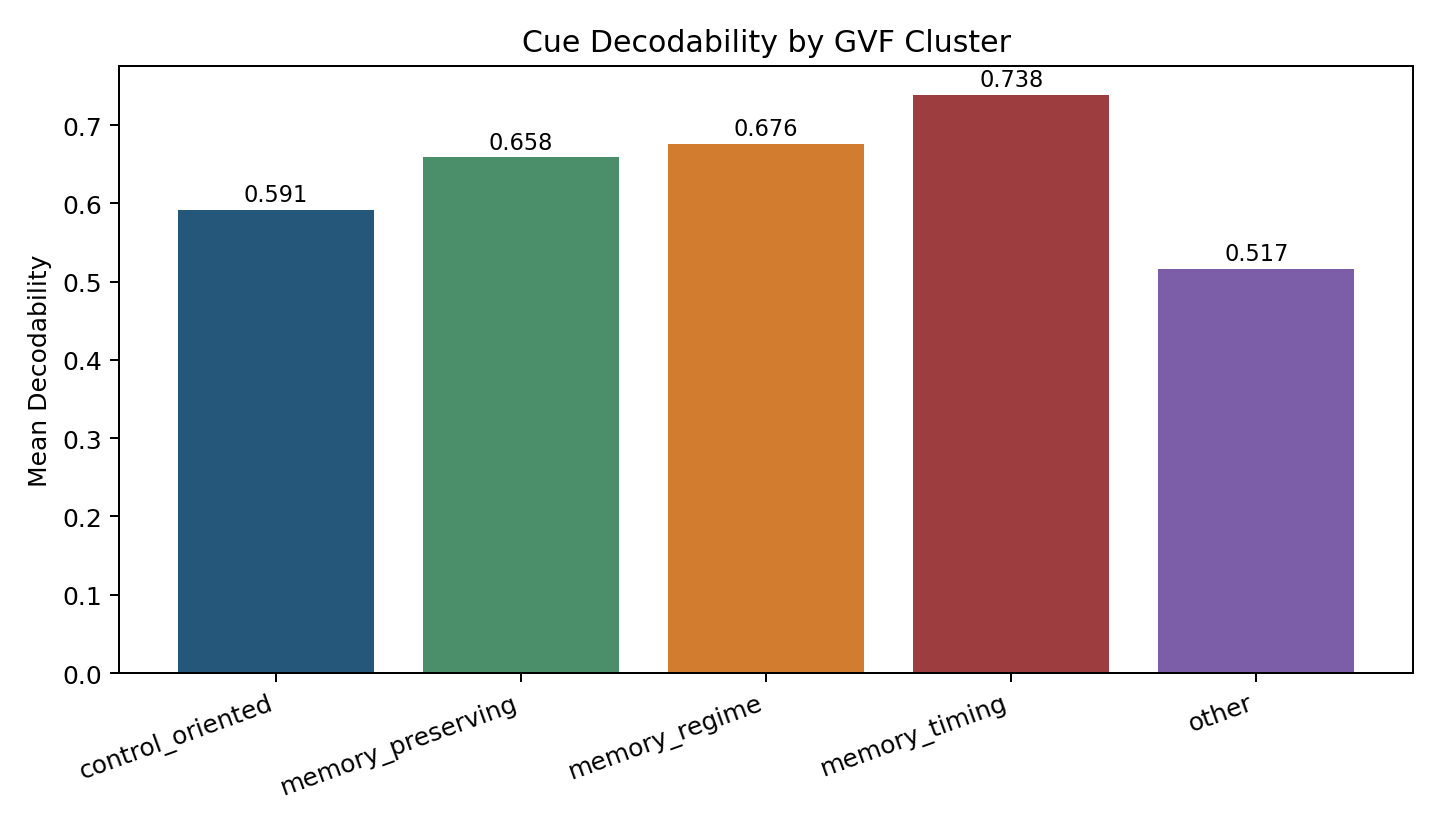
\includegraphics[width=0.7\linewidth]{figures/cluster_decodability.png}
\caption{Mean cue decodability by discovered GVF family.}
\label{fig:cluster_decodability}
\end{figure}

\begin{figure}[h]
\centering
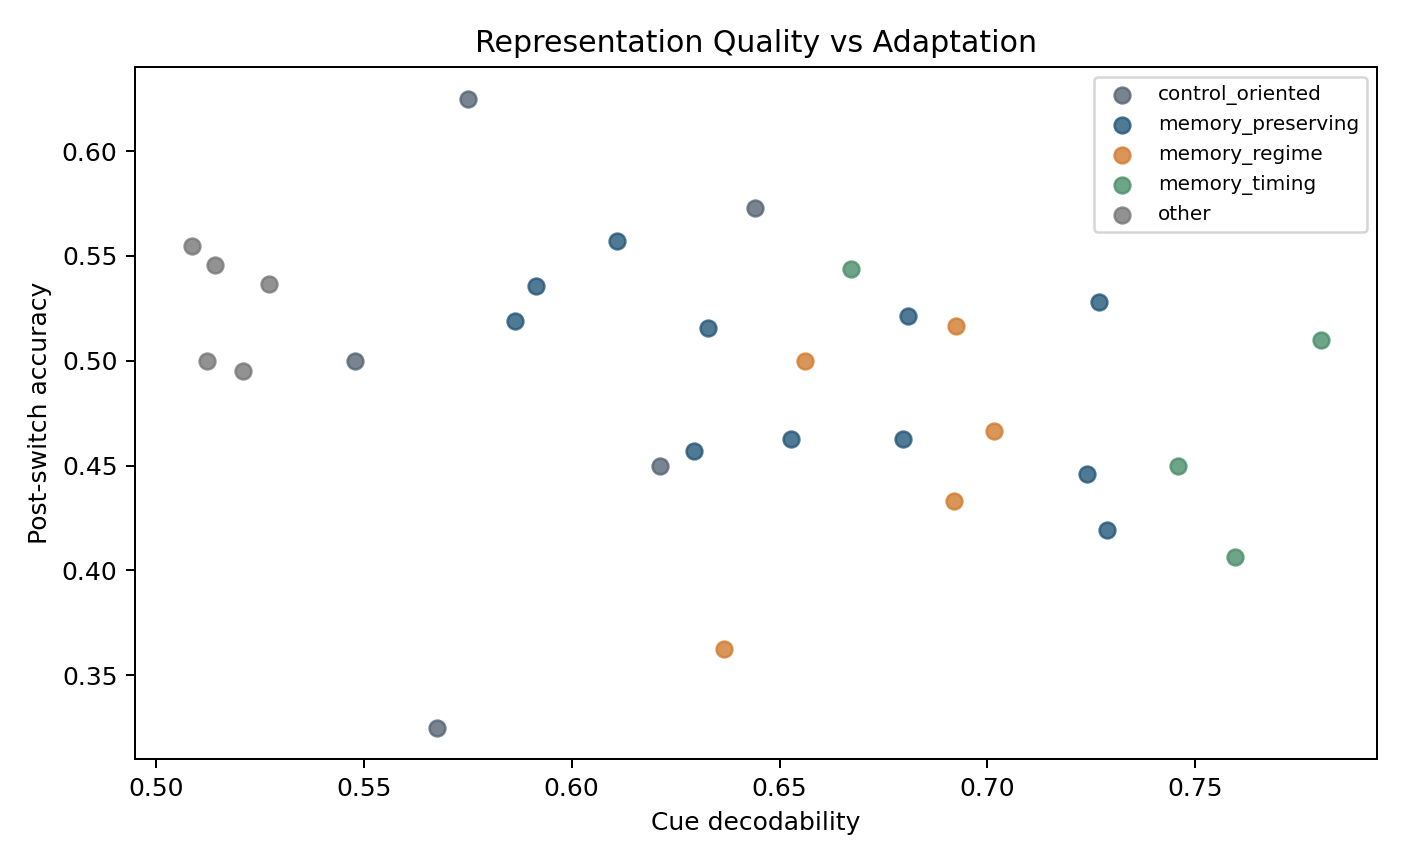
\includegraphics[width=0.78\linewidth]{figures/decodability_vs_adaptation.png}
\caption{Relationship between representation quality and adaptation across runs.}
\label{fig:decodability_vs_adaptation}
\end{figure}

\section{Additional Mechanism Evidence in the Big-World Benchmark}
\subsection{What the base method is learning}
Single-seed score traces show that \texttt{cue} remains the dominant best-scoring candidate across reselection points, while the second active GVF shifts from reward-like to timing-like support. This suggests that the generator is searching around a persistent memory core rather than merely overfitting one hand-designed primitive.

\subsection{Diversity-aware mixed GVFs}
Once diversity pressure is enabled, the evolutionary generator spends much of its occupancy on mixed families such as \texttt{mix:cue:time-to-junction} and \texttt{mix:cue:correct-turn}. This is mechanism evidence that the diversity term keeps semantically complementary candidates alive long enough to affect selection.

\subsection{Adaptive variants across severity}
We also ran an additional severity sweep for the drift-aware meta-heuristic bank.

\begin{table}[h]
\centering
\begin{tabular}{lcccc}
\toprule
Severity & Raw & Cue & Fixed bank & Drift-aware meta bank \\
\midrule
Mild post-switch & 0.5286 & 0.5333 & 0.6778 & 0.5071 \\
Moderate post-switch & 0.6929 & 0.5583 & 0.4875 & 0.5333 \\
Severe post-switch & 0.6000 & 0.5700 & 0.2250 & 0.5000 \\
\bottomrule
\end{tabular}
\caption{Two-seed severity sweep for the drift-aware meta-heuristic and comparison methods, from \texttt{results/meta\_bigworld\_sweep\_summary.csv}.}
\label{tab:metaseverity}
\end{table}

\begin{figure}[h]
\centering
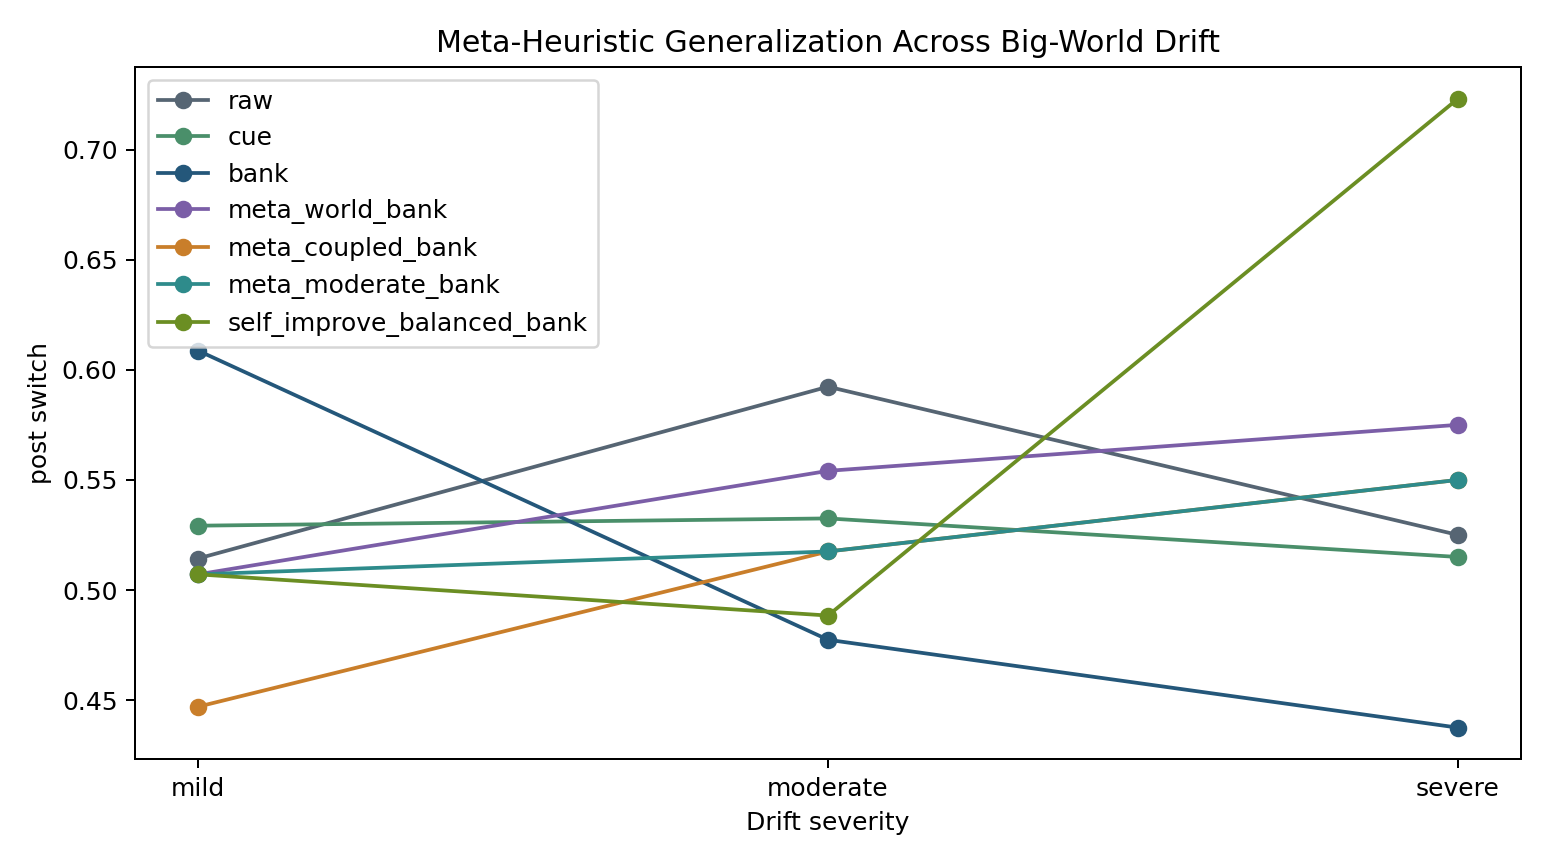
\includegraphics[width=0.8\linewidth]{figures/meta_bigworld_postswitch.png}
\caption{Post-switch adaptation across drift severity for raw, cue, fixed-bank, and drift-aware meta-bank methods.}
\label{fig:meta_bigworld_postswitch}
\end{figure}

These results are useful for diagnosis, but they mainly sharpen the same conclusion already retained in the main text: mild-world pruning helps, yet the central unresolved difficulty remains moderate-regime coupling control.

\subsection{Role reorganization under stronger drift}
The role occupancy analysis reveals that the learned bank reorganizes as the environment becomes harsher: \texttt{memory\_timing} occupancy decreases from 0.5106 in the mild setting to 0.4375 in the severe setting, while both \texttt{memory\_control} and \texttt{memory\_core} increase.

\begin{figure}[h]
\centering
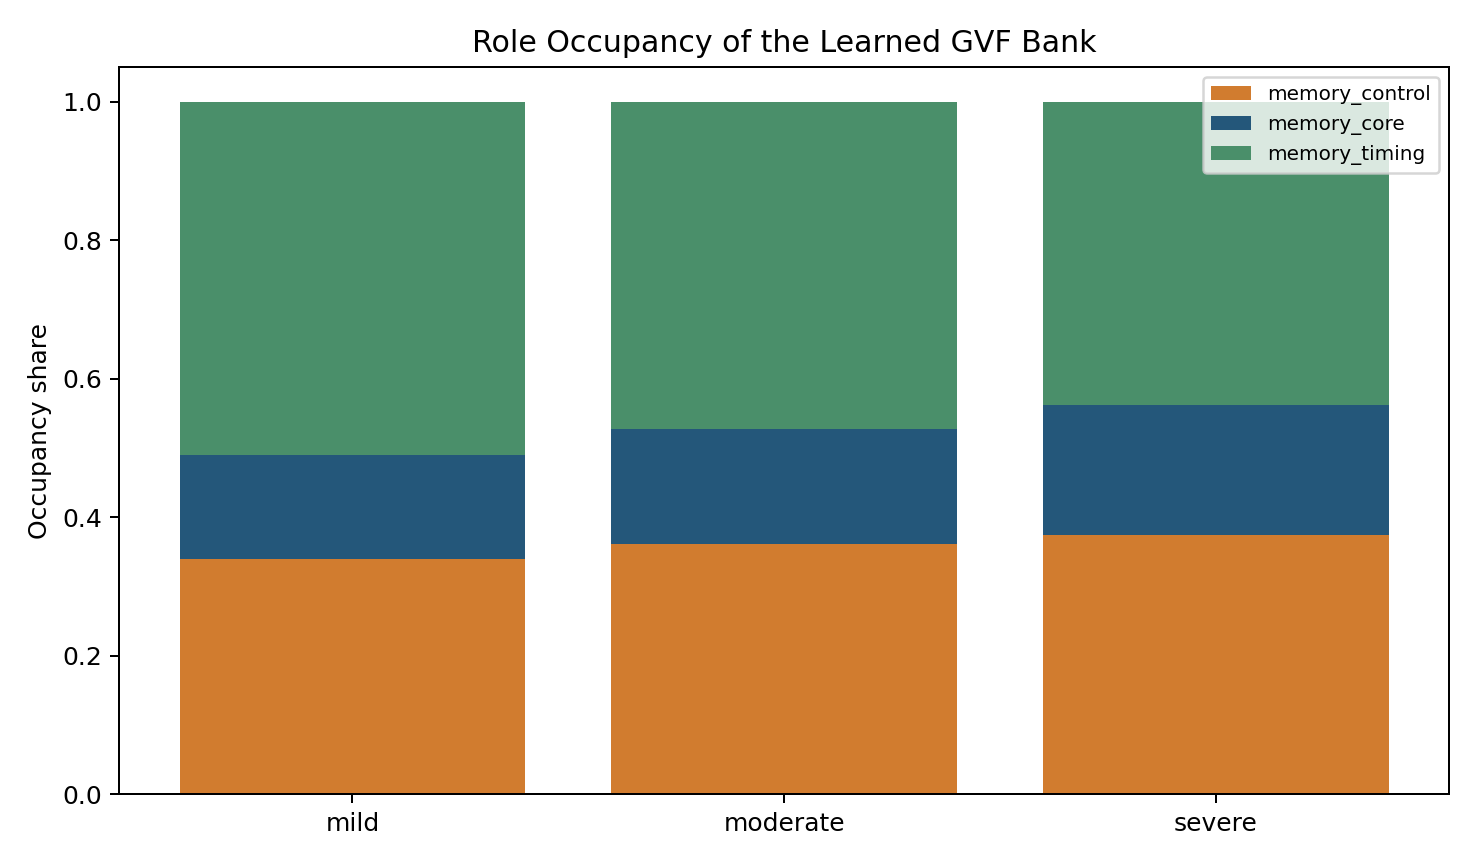
\includegraphics[width=0.78\linewidth]{figures/bigworld_role_occupancy.png}
\caption{Role occupancy of the learned GVF bank across drift severity.}
\label{fig:role_occupancy}
\end{figure}

\end{document}
